\chapter{UML}

I diagrammi UML permettono di descrivere graficamente l'applicazione sotto vari punti di vista, garantendo la comprensione del funzionamento del software, delle esigenze che esso soddisfa e delle relazioni che intercorrono fra i suoi componenti.

TODO FORSE ALLUNGARE IL BRODO.

\section{Use case diagram}

\begin{figure}[H]
    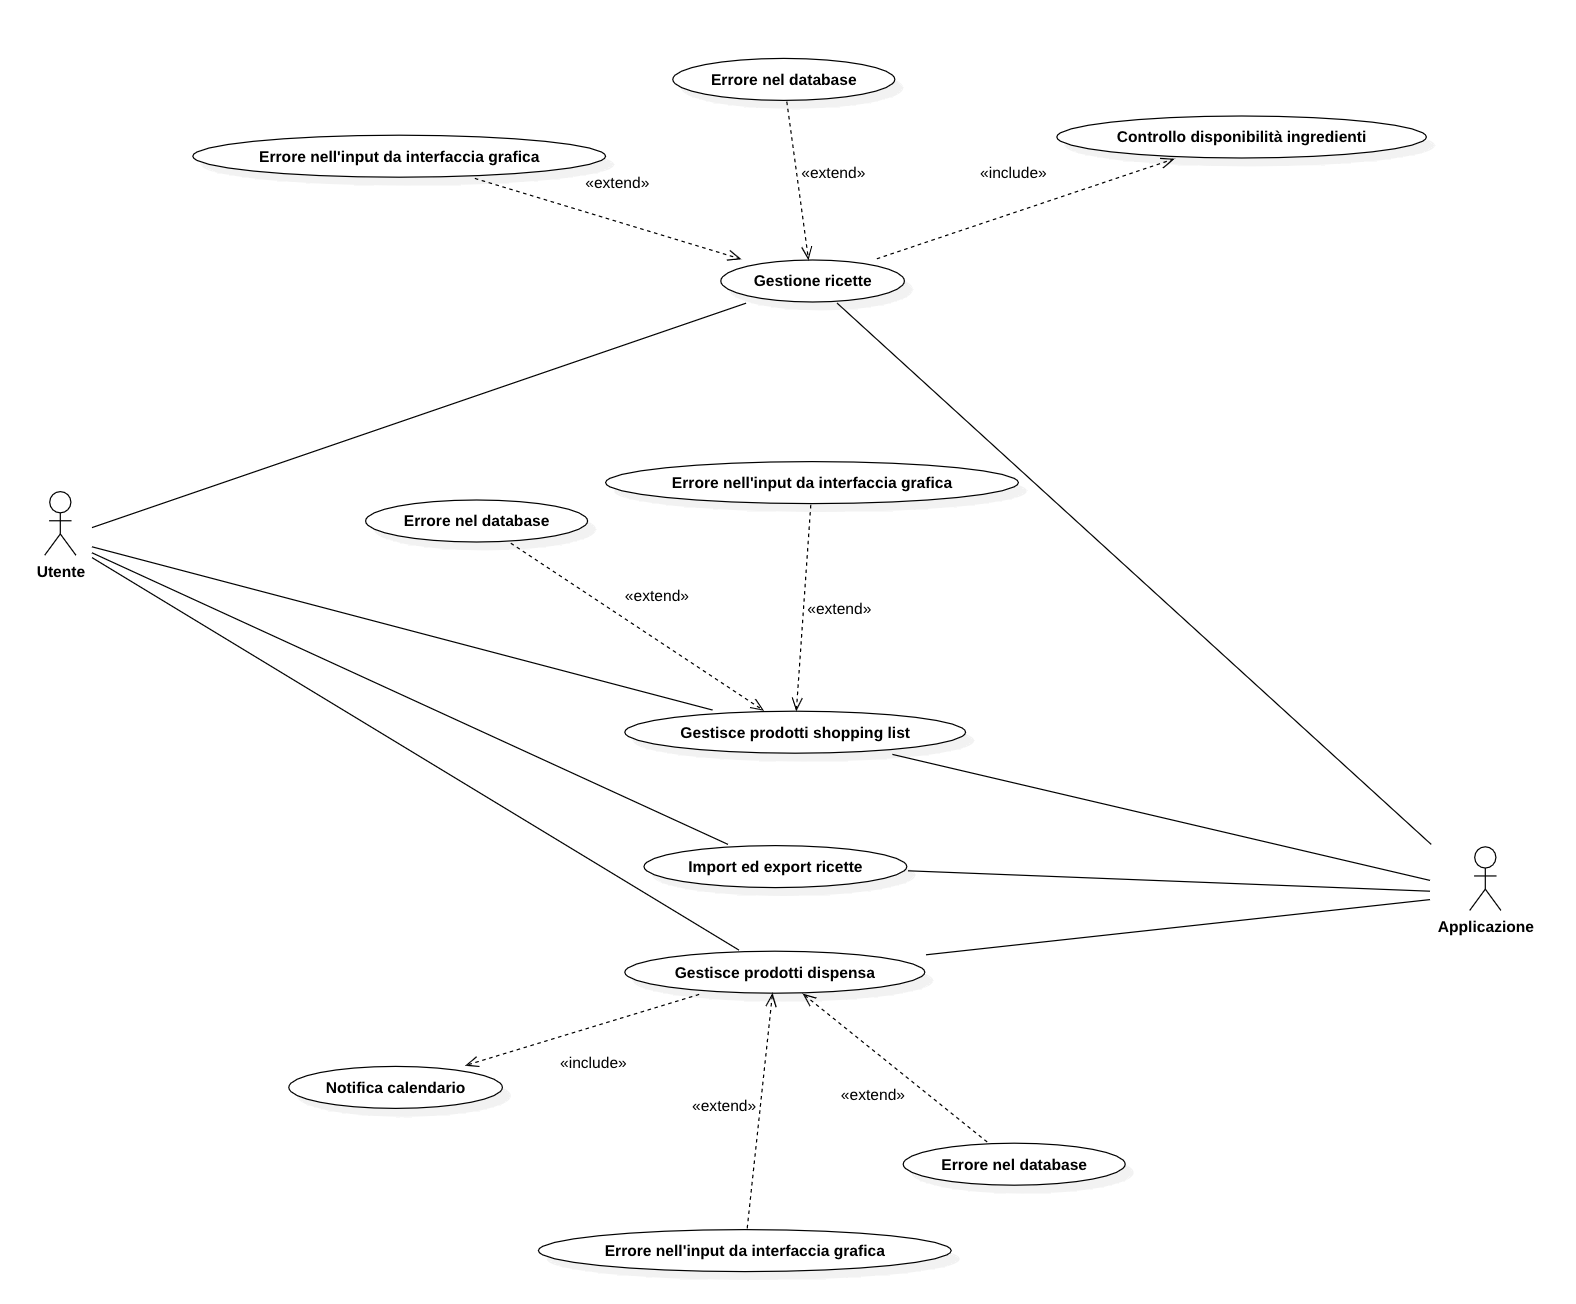
\includegraphics[width=\linewidth]{images/use-case.png}
    \caption{Diagramma dei casi d'uso.}
    \label{fig:usecase}
\end{figure}

Lo use case diagram permette di identificare gli attori che interagiscono col sistema e le attività che essi possono svolgere. Lo scopo è descrivere le principali funzionalità del software.

TODO FORSE ALLUNGARE IL BRODO.

\newpage

\section{Activity diagram}

L'activity diagram consente di specificare come il sistema realizzerà le funzionalità mostrate nello use case. Lo scopo è connettere tra loro azioni di alto livello per rappresentare un processo che viene svolto nel sistema. Per una migliore comprensione del funzionamento, nei diagrammi seguenti si è scelto di non modellare i casi di errore del database e dell'interfaccia grafica. 

\subsection{Activity diagram della dispensa}

In questo diagramma viene mostrato il processo relativo all'interazione fra l'utente e l'applicazione per la gestione della dispensa. 

\begin{figure}[H]
    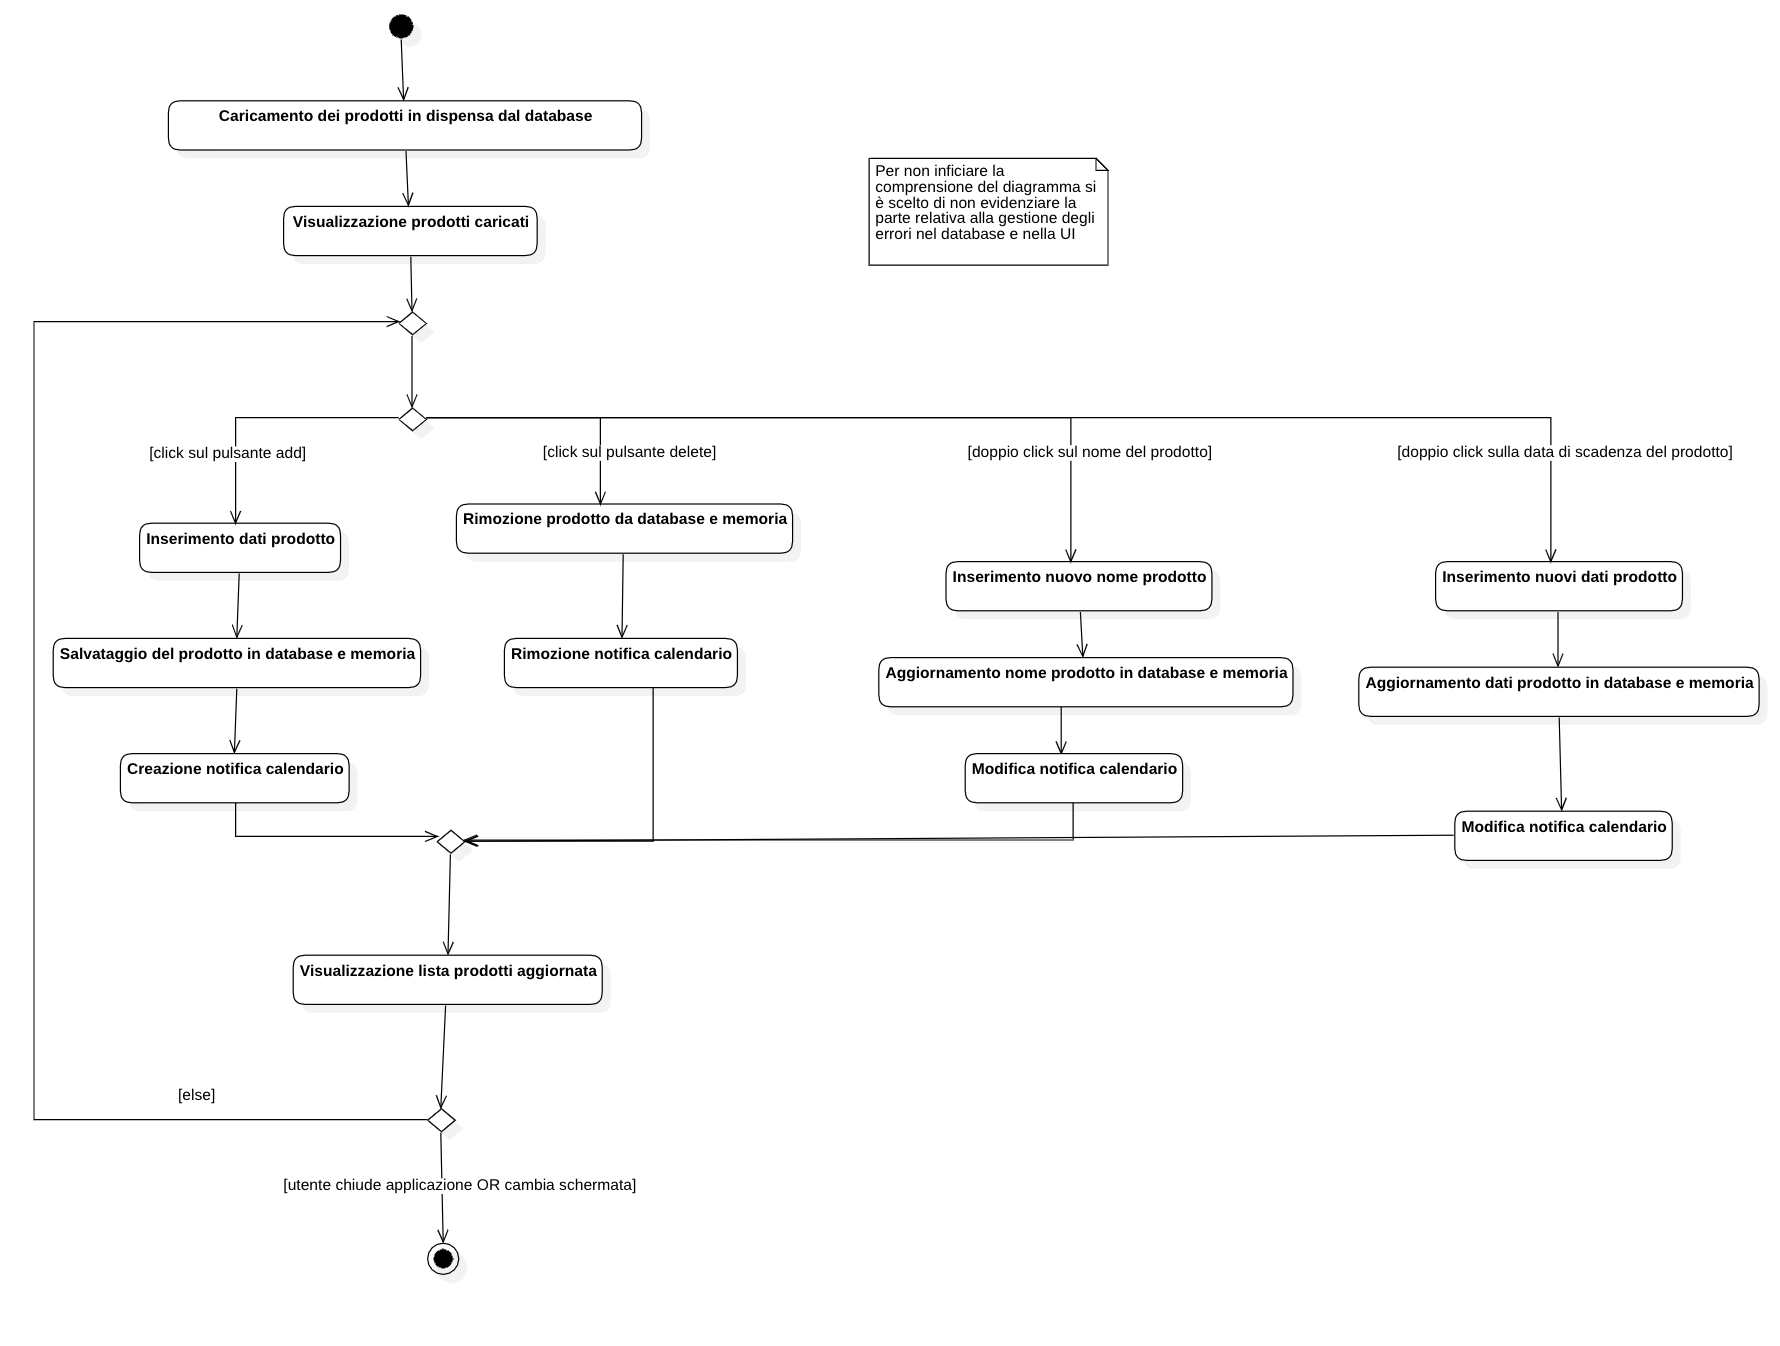
\includegraphics[width=\linewidth]{images/activity-pantry.png}
    \caption{Diagramma delle attività della dispensa.}
    \label{fig:actpantry}
\end{figure}

TODO FORSE ALLUNGARE IL BRODO.

\newpage

\subsection{Activity diagram della lista della spesa}

In questo diagramma viene mostrato il processo relativo all'interazione fra l'utente e l'applicazione per la gestione della lista della spesa.

\begin{figure}[H]
    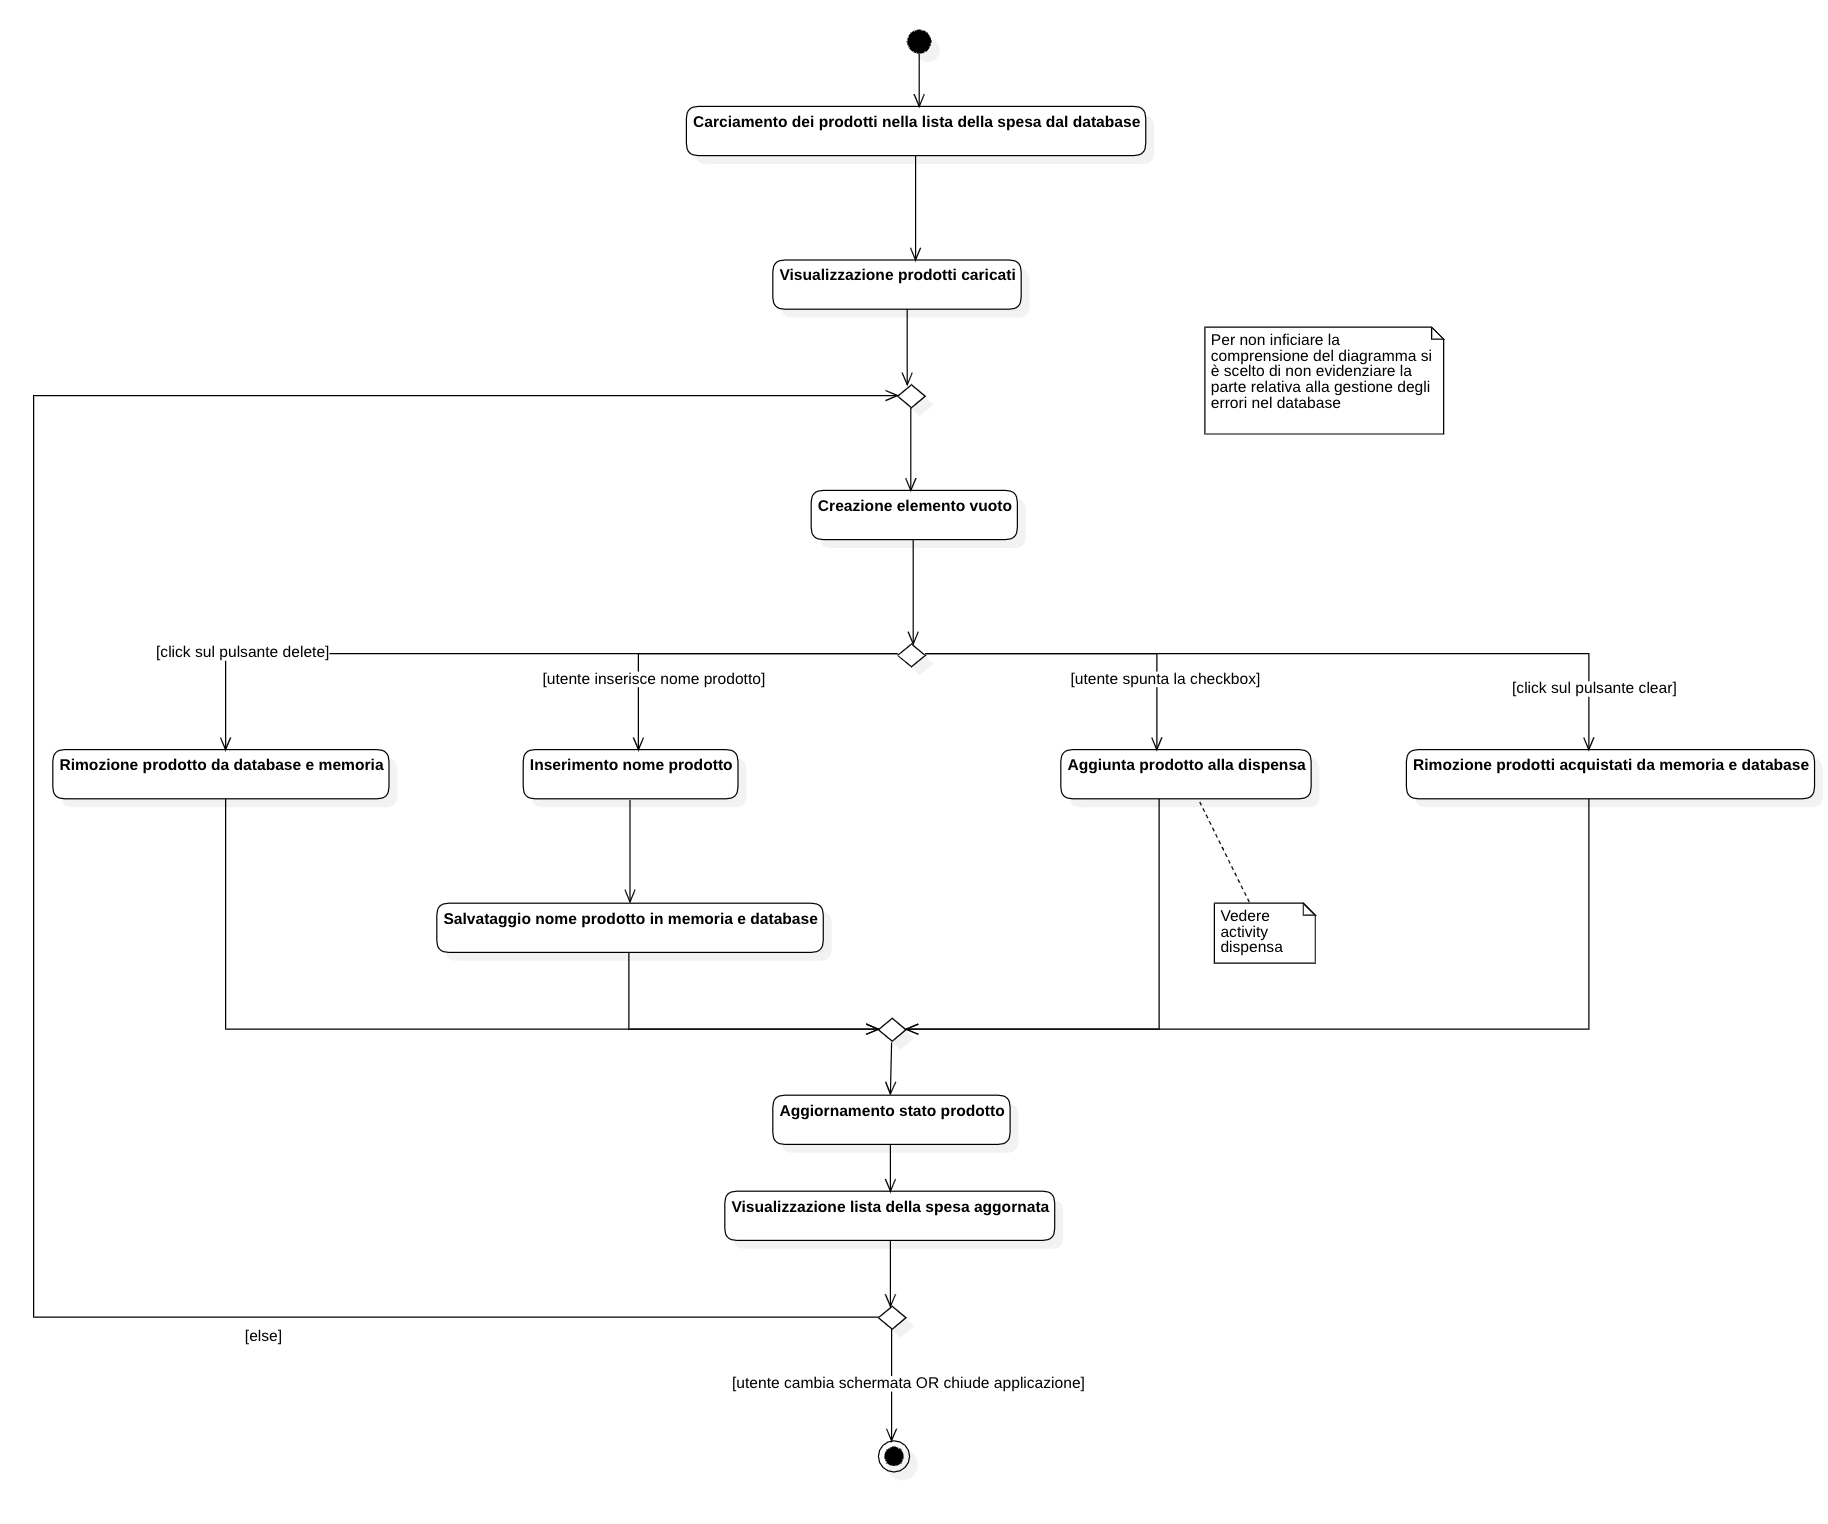
\includegraphics[width=\linewidth]{images/activity-shopping-list.png}
    \caption{Diagramma delle attività della lista della spesa.}
    \label{fig:actshoplist}
\end{figure}

TODO FORSE ALLUNGARE IL BRODO.

\newpage

\subsection{Activity diagram delle ricette}

In questo diagramma viene mostrato il processo relativo all'interazione fra l'utente e l'applicazione per la gestione delle ricette, inclusa la possibilità di importare ed esportare ricette.

\begin{figure}[H]
    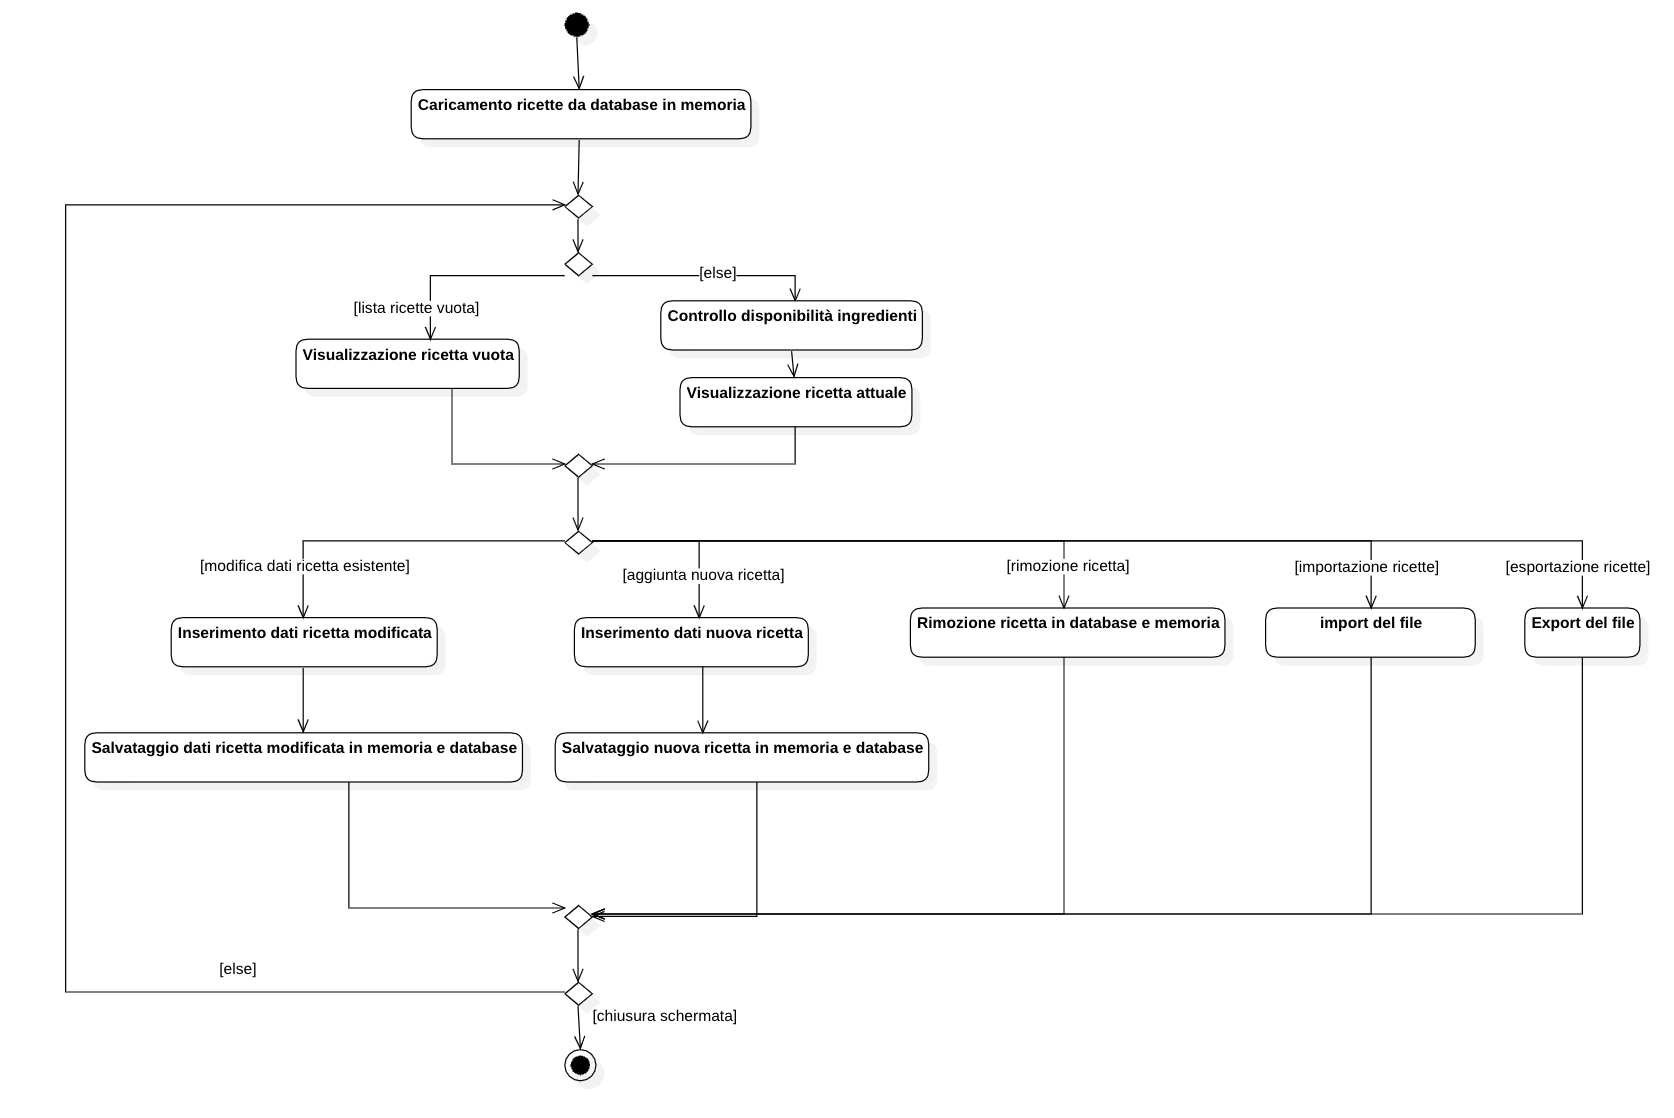
\includegraphics[width=\linewidth]{images/activity-recipe.png}
    \caption{Diagramma delle attività delle ricette.}
    \label{fig:actrecipe}
\end{figure}

TODO FORSE ALLUNGARE IL BRODO.

\newpage

\section{State diagram}

Lo state diagram permette di modellare gli stati in cui si trova un oggetto e gli eventi che causano le transizioni fra gli stati. 

\subsection{State diagram della ricetta}

In questo diagramma vengono mostrati gli stati in cui si può trovare una ricetta in base alla presenza, e alla disponibilità, degli ingredienti.

\begin{figure}[H]
    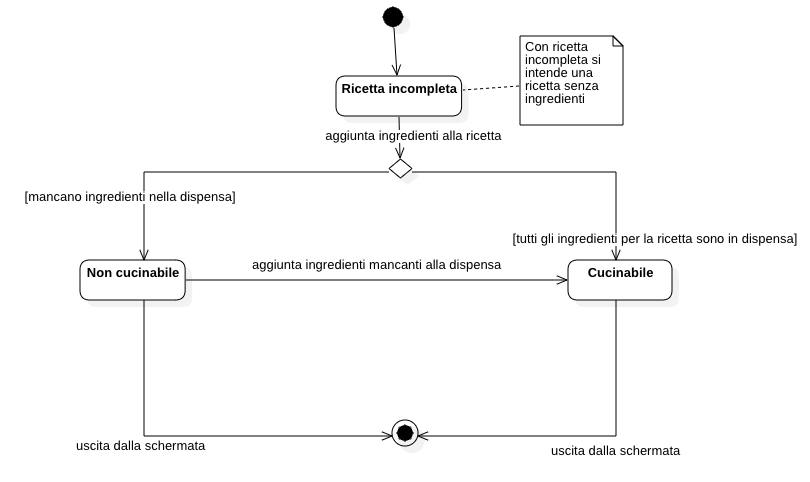
\includegraphics[width=\linewidth]{images/state-recipe.png}
    \caption{Diagramma degli stati della ricetta.}
    \label{fig:staterecipe}
\end{figure}

TODO FORSE ALLUNGARE IL BRODO.

\newpage

\subsection{State diagram della lista della spesa}

In questo diagramma vengono mostrati gli stati in cui si può trovare un prodotto presente nella lista della spesa.

\begin{figure}[H]
    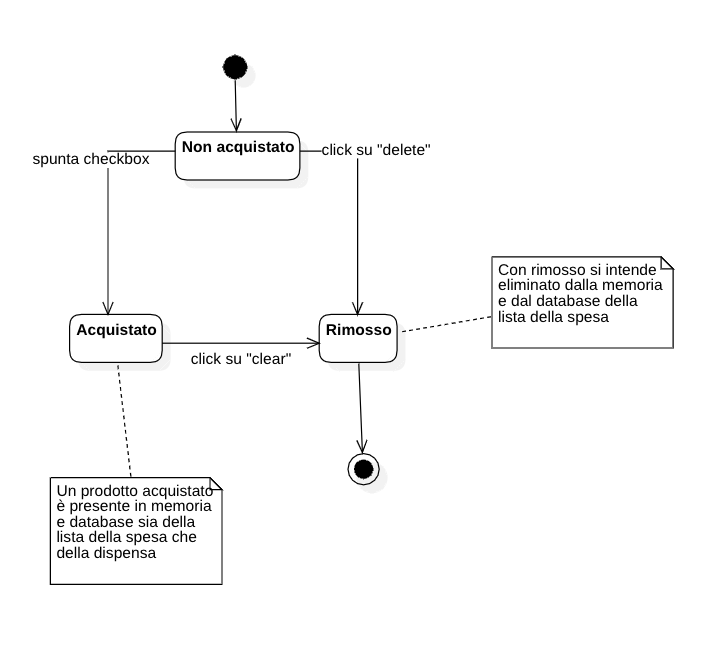
\includegraphics[width=\linewidth]{images/state-shopping-list.png}
    \caption{Diagramma degli stati della lista della spesa.}
    \label{fig:stateshoplist}
\end{figure}

TODO FORSE ALLUNGARE IL BRODO.

\newpage

\section{Class diagram}

Il class diagram permette di descrivere i tipi di oggetti presenti nel sistema e le relazioni statiche che intercorrono tra di essi. Esso descrive inoltre gli attributi e i metodi di ogni classe, oltre ai vincoli che si applicano nel collegamento tra gli oggetti.

\begin{figure}[H]
    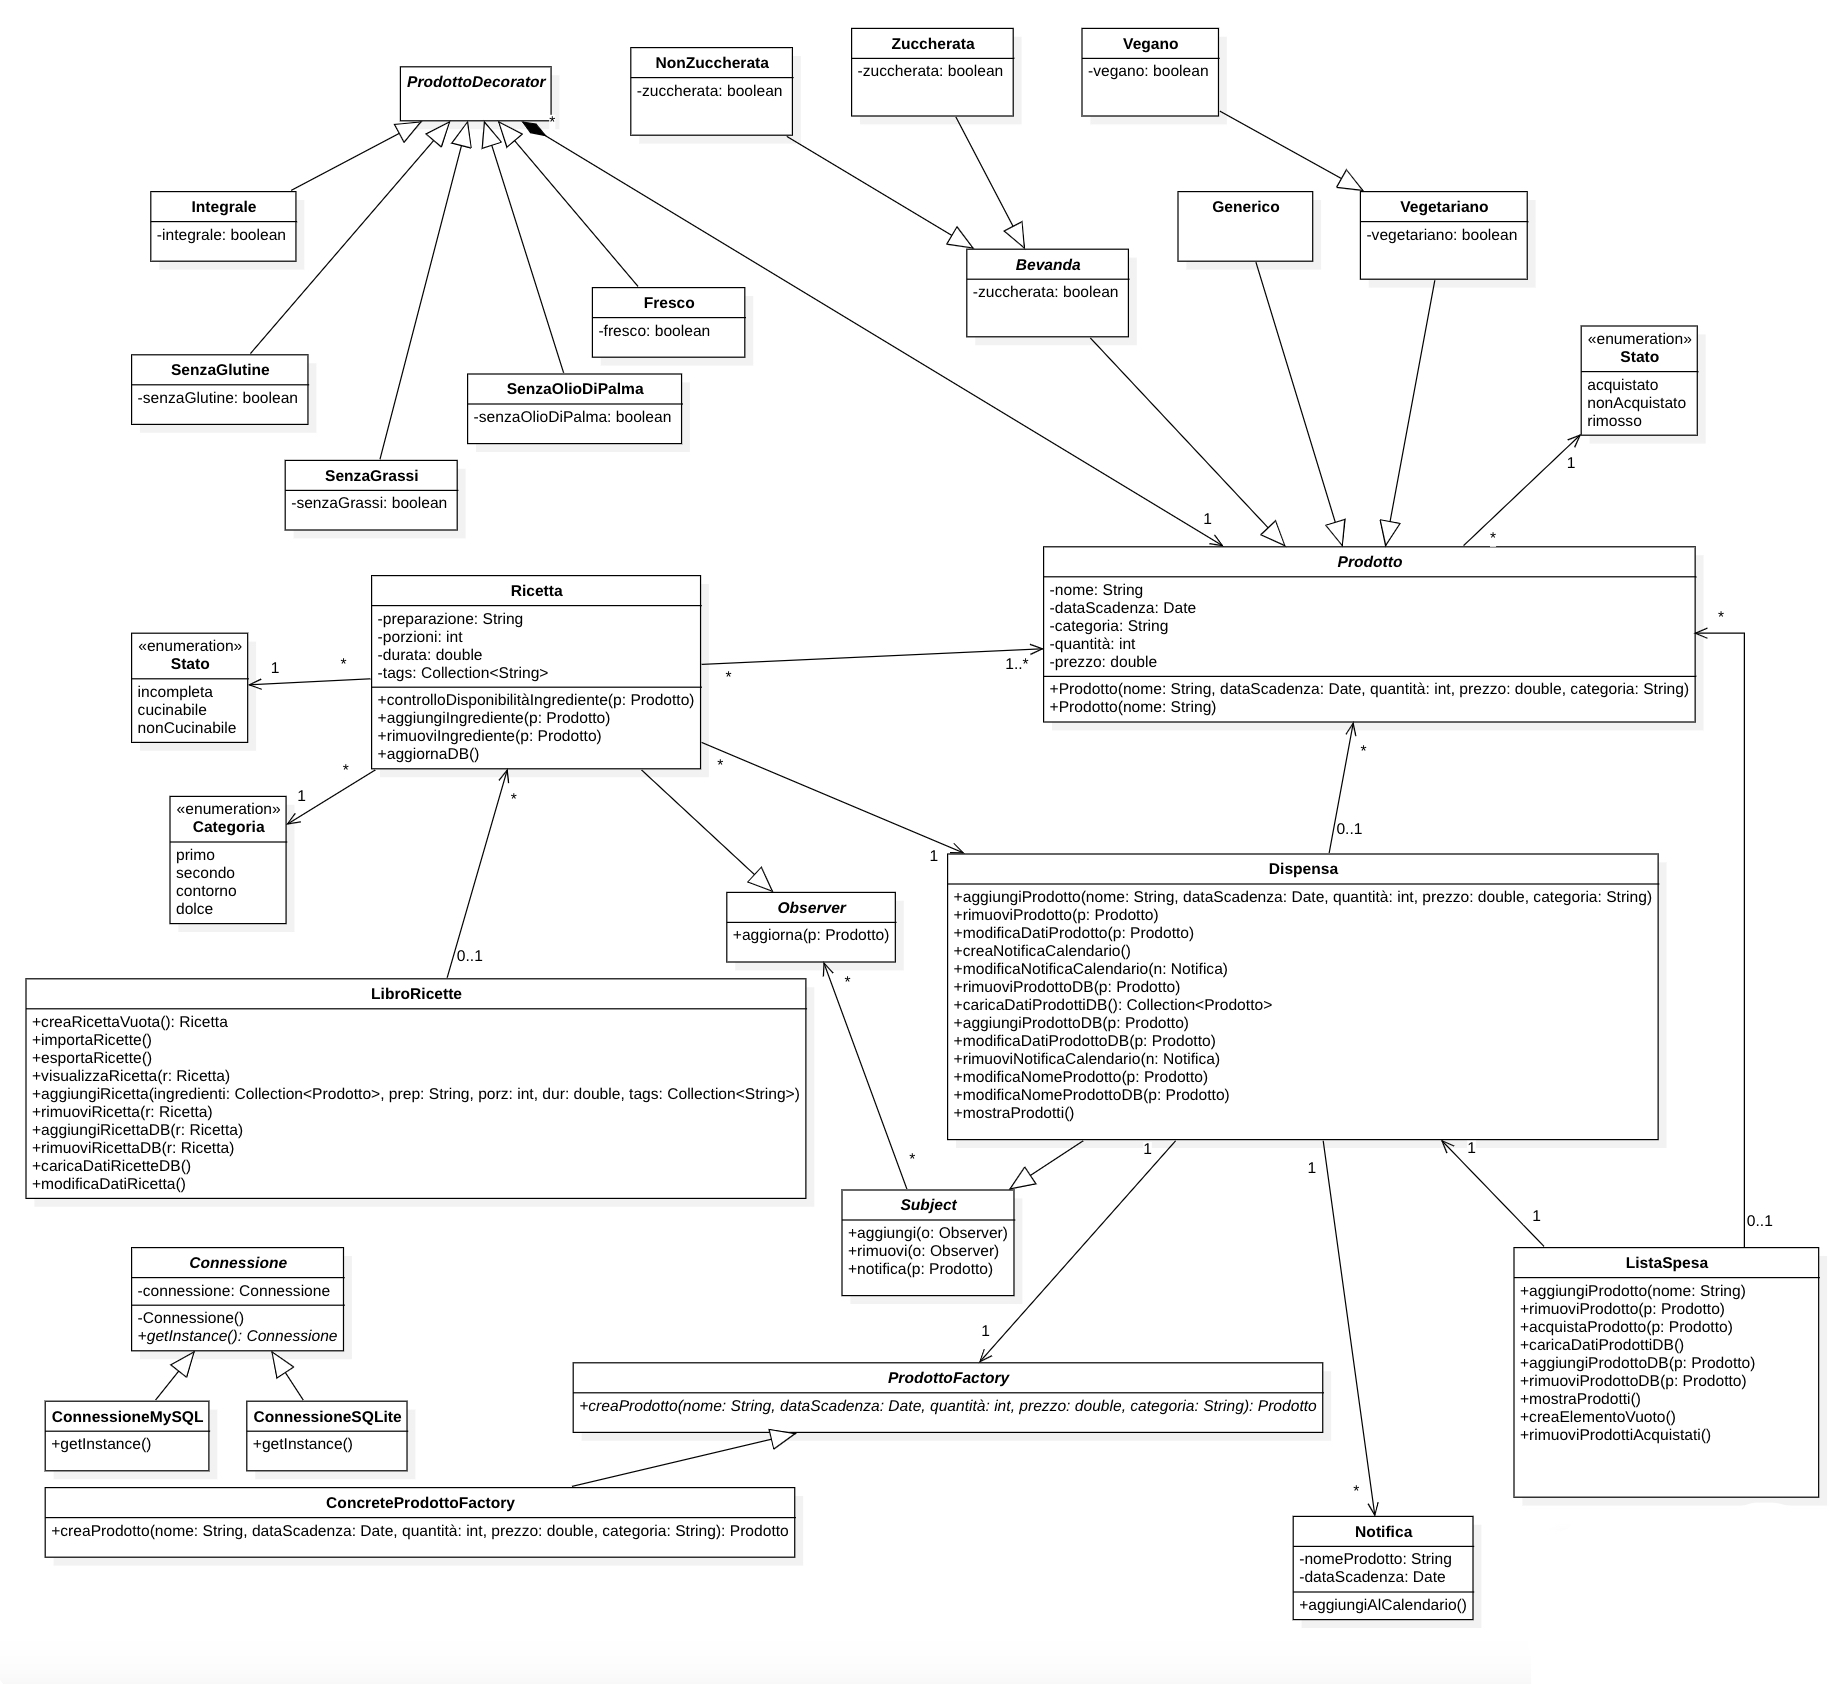
\includegraphics[width=\linewidth]{images/class.jpeg}
    \caption{Diagramma delle classi.}
    \label{fig:classdiagram}
\end{figure}

Per non complicare ulteriormente il diagramma si è scelto di non rappresentare la parte relativa all'interfaccia grafica. I design pattern applicati verranno spiegati nella sezione corrispondente.

\newpage

\section{Sequence diagram}

Il sequence diagram serve per descrivere singoli scenari dell'applicazioni. Lo scopo è mostrare come il sistema svolge le proprie funzioni. Per una migliore comprensione del funzionamento, nei diagrammi seguenti si è scelto di non modellare i casi di errore del database e dell'interfaccia grafica. 

TODO ALLUNGARE IL BRODO.

\subsection{Sequence diagram della dispensa}

\begin{figure}[H]
    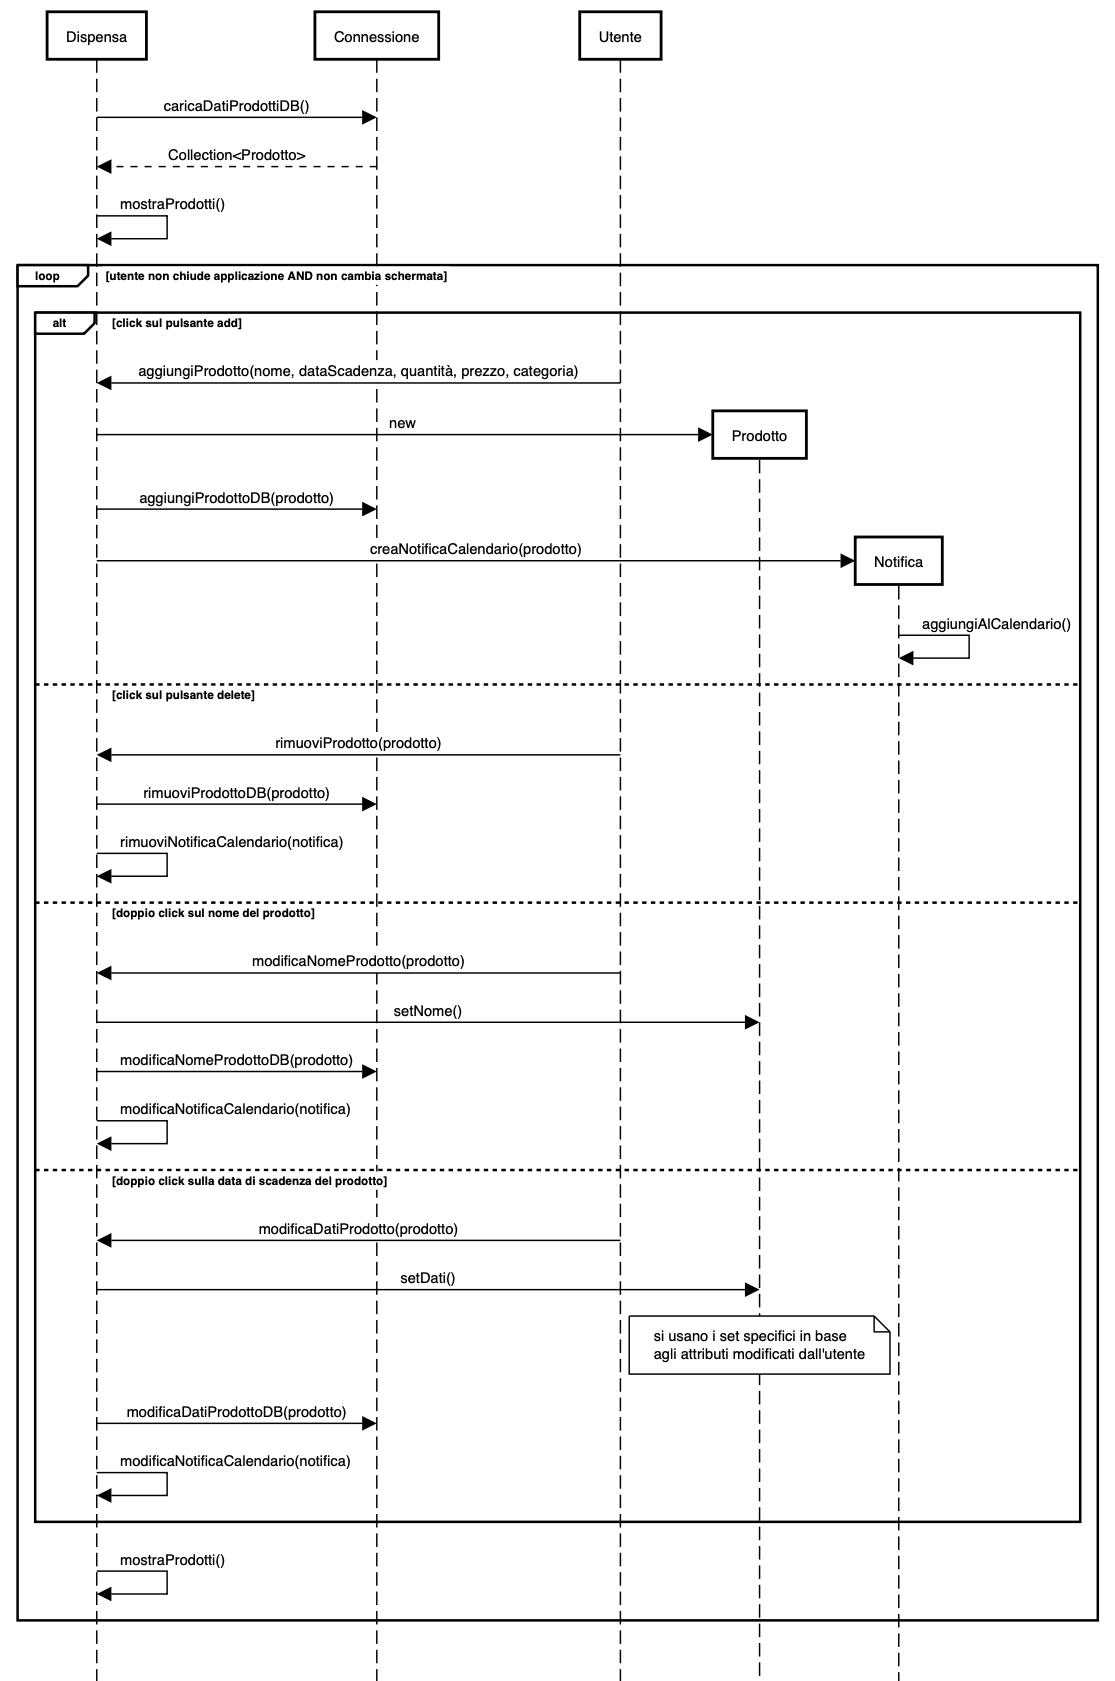
\includegraphics[width=\linewidth]{images/sequence-pantry.png}
    \caption{Diagramma di sequenza della dispensa}
    \label{fig:seqpantry}
\end{figure}

\subsection{Sequence diagram della lista della spesa}

\begin{figure}[H]
    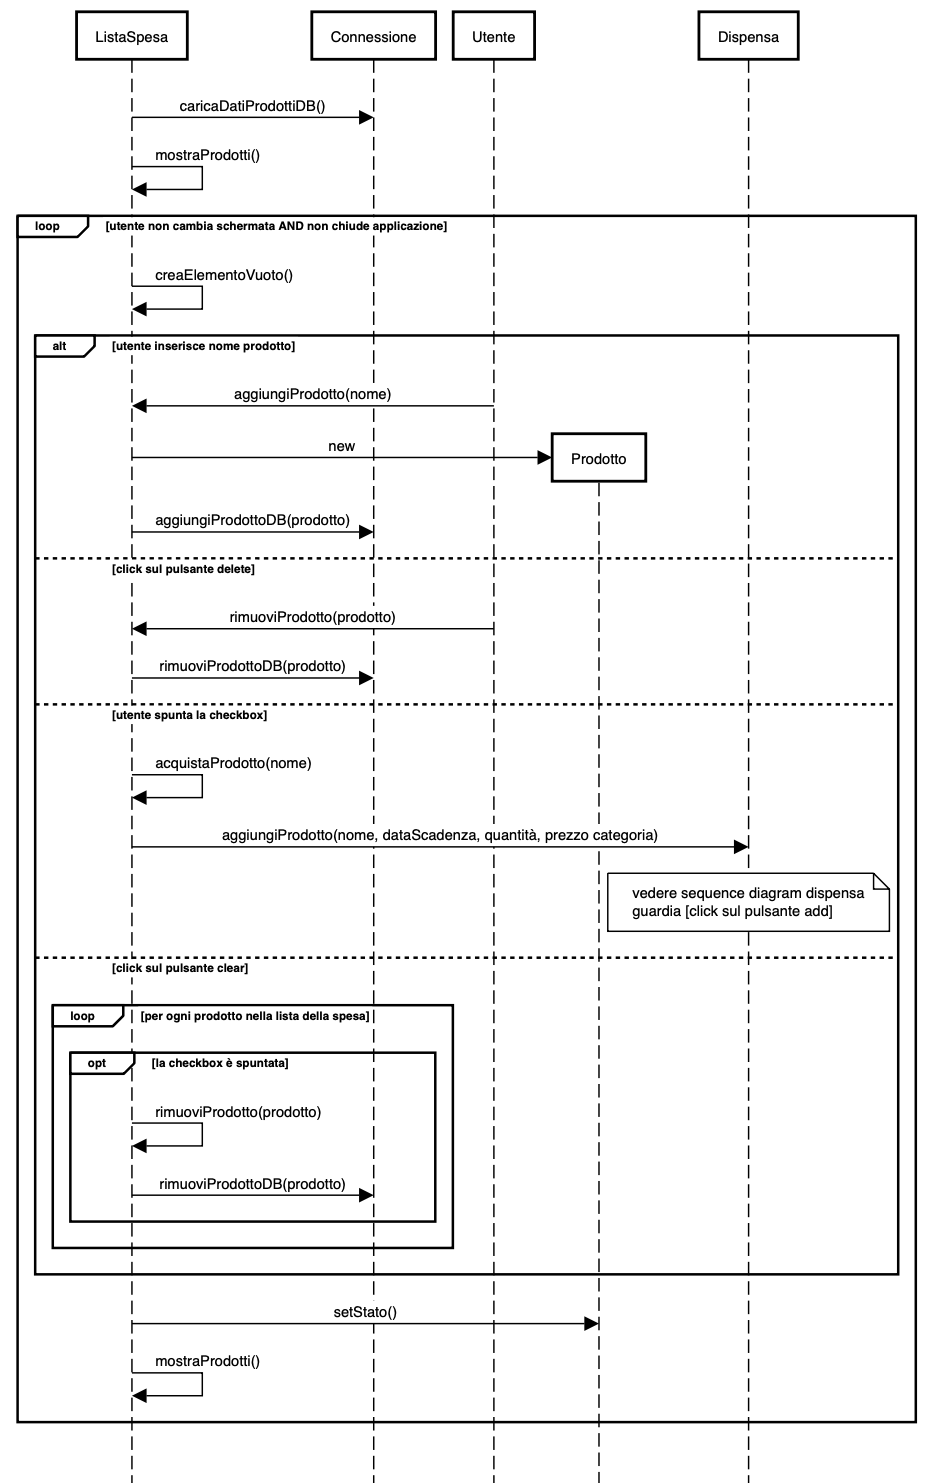
\includegraphics[width=\linewidth]{images/sequence-shopping-list.png}
    \caption{Diagramma di sequenza della lista della spesa}
    \label{fig:seqshoplist}
\end{figure}

\subsection{Sequence diagram delle ricette}

\begin{figure}[H]
    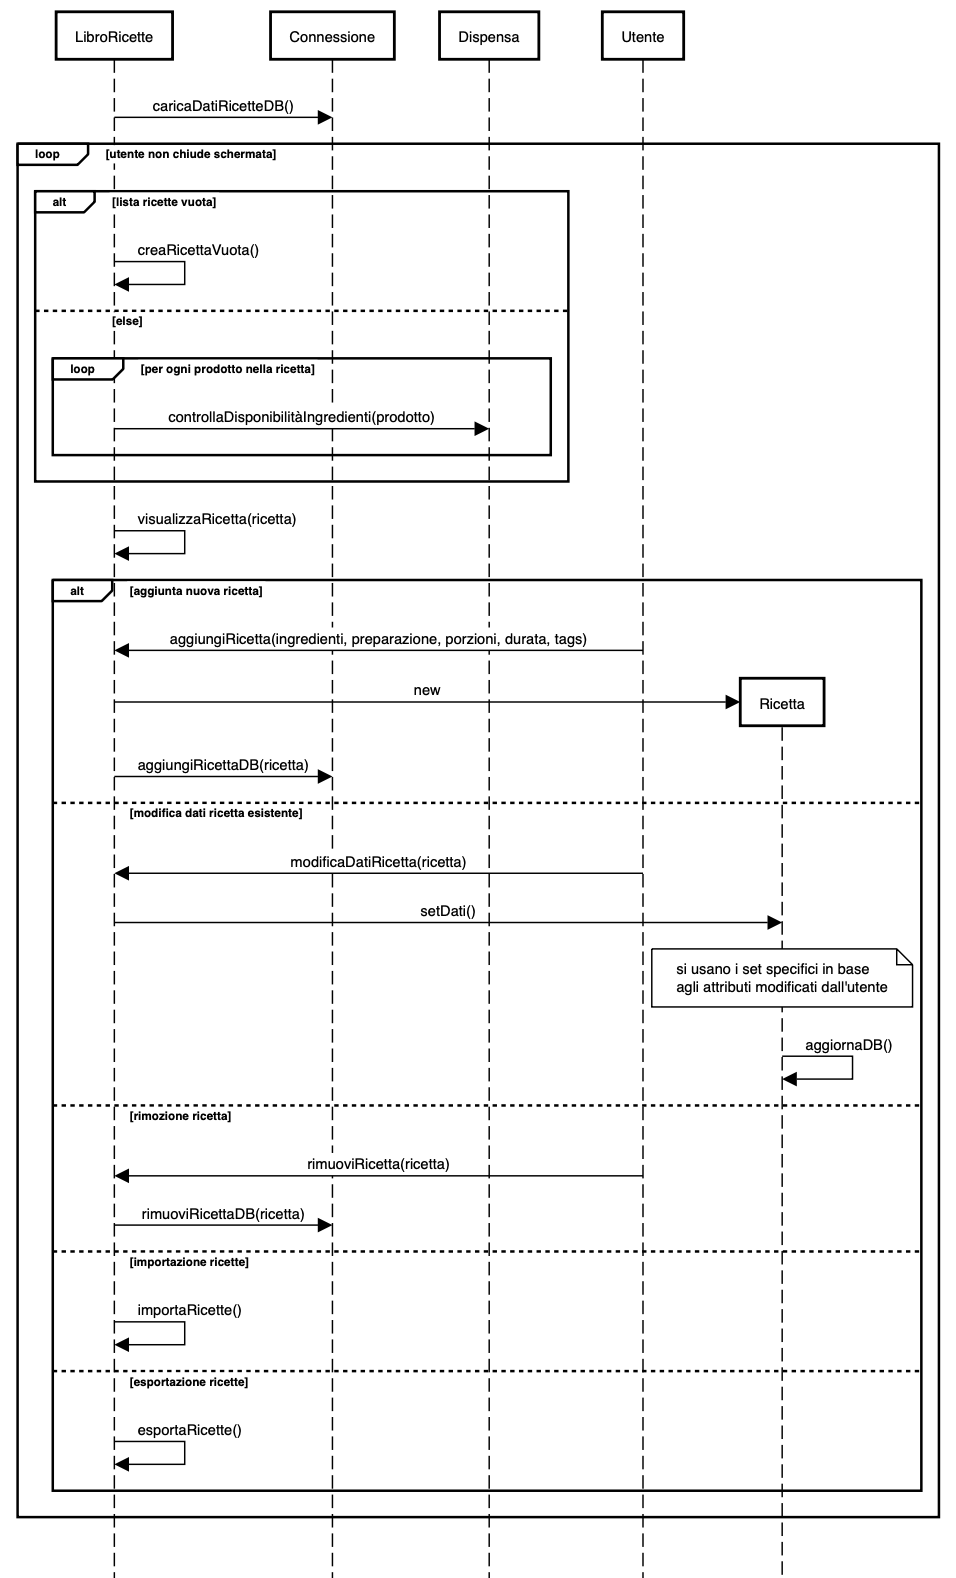
\includegraphics[width=\linewidth]{images/sequence-recipe.png}
    \caption{Diagramma di sequenza delle ricette}
    \label{fig:seqrecipe}
\end{figure}

Si noti che, per evitare sovrapposizioni nel diagramma che ne avrebbero resa più difficile la comprensione, il metodo \inlinecode{Java}{creaRicettaVuota()} (che si limita a mostrare dei campi di testo vuoti all'utente tramite l'interfaccia grafica) non crea un oggetto di tipo Ricetta (come invece avviene nel caso del metodo \\ \inlinecode{Java}{aggiungiRicetta(ingredienti, preparazione, porzioni, durata, tags)} in cui la ricetta creata presenta valori non nulli nei propri attributi).

